%! TEX root = ./master.tex

\lecture{Ch. 3 continue}{2020-09-23}{Representing Integers}

\paragraph{Sign extension}
Given a $w$ bit signed integer $x$, convert it to a $w + k$ bit signed integer with the same value.
.
We do that by coping the most significant bit of $x$ and copy it to all $k$ new bits

\paragraph{Truncation}
Throws away the left bits. For unsigned numbers it represents the modulo operator. For signed integers it is also like modulo, but it dies it in a special way (negative number may get positive and vice versa).

\subsubsection{Integer addition and subtraction in C}

Convert get negative number of $x$ using $\tilde x + 1 == -x$.

The complement of $x$ is $\tilde x$ and $\tilde x + x == 111 \dots 111 == -1$

\paragraph{Unsigned addition}
The function $UAdd_w(u,v)$ ignores the extra bit which would be required if the sum overflows the $w$ bits.

There are certain compilers which provide some possibility to retrieve a possible overflow.

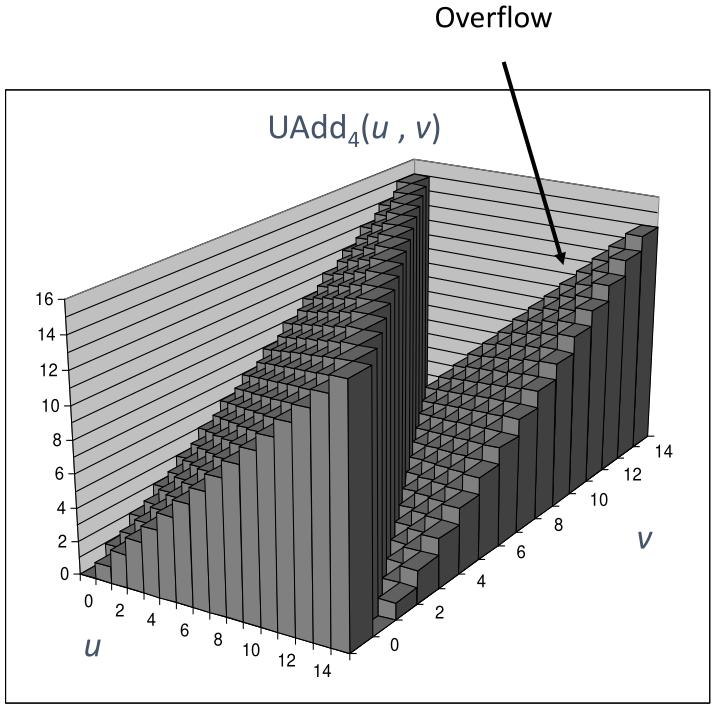
\includegraphics[width=0.8\textwidth]{04_01_unsignedAddition.png}

$UAdd_w(u,v)$ is an Abelian group (Closed, Commutative, Associative, Identity, Inverse)

\paragraph{Two's complement addition}
$TAdd_w(u,v)$ behaves identical to $UAdd$ in the bit level interpretation. But the overflow behaves differently. Positive overflow gives a negative number, a negative overflow gives a positive number.Positive overflow gives a negative number, a negative overflow gives a positive number.

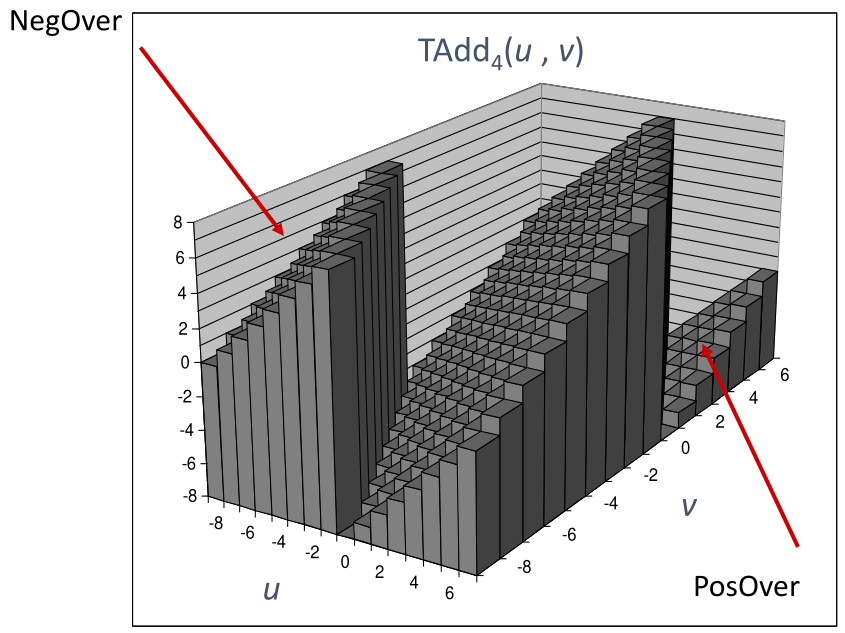
\includegraphics[width=0.8\textwidth]{04_02_signedAddition.png}
 
$TAdd$ is isomorphic to $UAdd$ and $TAdd$ forms a group (closed, commutative, associative, identity, inverse).

\subsubsection{Integer multiplication in C}

\paragraph{Unsigned multiplication}
The range is $0 \le x \cdot y \le (2^w -1)2$

The operator $UMult_w(u,v)$ truncates the overflowing bits and it forms a commutative ring with $UAdd$.

\paragraph{Two's complement multiplication}
The lowest number $x \cdot y \ge (-2^{w - 1}) \cdot (2^{w - 1} - 1)$

The greatest number $x \cdot y \le (-2^{w -1})^2$

The operator $TMult_w(u,v)$ ignores the overflowing bits. Some hardware puts overflowing bits into a special register, but they are normally not accessibly in C.


\paragraph{Integer multiplication and division using shifts}
$u << k$ gives $u \cdot 2^k$ for signed and unsigned numbers.

Multiplication is much more complex than simple shifts. Therefore, to calculate $u \cdot 24$ we may write $(u << 5) - (u << 3)$. But modern compiler do such thinks (and even better optimisations) for us, therefore we should not do it.

$u >> k$ gives $\lFloor \frac{u}{2^k} \rFloor$ (we truncate all digits overflowing on the right) for unsigned and signed numbers. But for signed numbers the results may be wrong for negative numbers because we round down, but actually we would like to round towards $0$. We fix that by computing $\lFloor \frac{(s + 2^k - 1)}{2^k} \rFloor$. In C this is equivalent to $(s + (1 << k) -1) >> k$.

If the compiler checks for signed number of the number is negative and does the devision depending on that.

\subsubsection{C Integer puzzles}


